\section{Monte Carlo}
\label{sec:mc}

The econometrician sees only $(y, X, Z)$. Each design draws $n$ observations from a known law $f_0$; the method and the baselines are run on the same data; recovery, errors and the diagnostic are recorded per run. Every search's Pareto front was saved, so the selection rules were compared afterwards on the same fronts.

\subsection{Designs, laws and metrics}
\label{sec:mc-design}

\begin{table}[ht]
\centering\small
\caption{Monte Carlo designs. $Z, v, \varepsilon \sim N(0,1)$ independent unless stated; default $\pi = 1$, $\rho = 0.8$; the strong-endogeneity setting has $\pi = 0.7$, $\rho = 1.2$.}
\label{tab:designs}
\begin{tabular}{@{}>{\raggedright\arraybackslash}p{3.0cm}>{\raggedright\arraybackslash}p{5.9cm}>{\raggedright\arraybackslash}p{5.3cm}@{}}
\toprule
Design & Data-generating process & Purpose \\
\midrule
D1 Confounding & $X = \exp(\pi Z + v)$; $u = \rho v + \sigma\varepsilon$ & Baseline; $X > 0$ so log and power laws are defined; $\E[y \mid X]$ has an extra $\frac{\rho}{1 + \pi^2}\log X$ term; control-function assumptions hold \\
D2 Heteroskedastic first stage & $X = \exp(\pi Z + \sigma(Z)v)$, $\sigma(Z) = e^{\gamma Z}$, $\gamma = 0.3$ & IV condition holds; the control function fails, since $\E[u \mid \hat v, Z] = \rho\hat v/\sigma(Z)$ depends on~$Z$ \\
D3 Simultaneity & $y = f_0(X) + u$ (supply, increasing) and $y = -\kappa\log X + \gamma Z + e$ (demand, shifted by $Z$); equilibrium $X$ solved numerically & Endogeneity from equilibrium, not from an omitted variable \\
D4 Discrete instrument & $Z$ uniform on $J = 4$ points & Restricted identification with few support points (\res{Proposition}{4}) \\
D5 Weak instrument & D1 with $\pi = 0.1$ & The method should report weak identification rather than a formula \\
\bottomrule
\end{tabular}
\end{table}

\begin{table}[ht]
\centering\small
\caption{Laws. ``In a finite library'' asks whether sparse IV over a fixed dictionary can represent the law.}
\label{tab:laws}
\begin{tabular}{@{}llll@{}}
\toprule
Law & Formula & Constants & In a finite library? \\
\midrule
Log & $1 + 2\log x$ & 2 & Yes \\
Power & $2x^{0.7}$ & 2 & No: nonlinear in $\theta$ \\
Kink & $x - 0.8\max(x - 1.5, 0)$ & 3 & No: unknown knot \\
Saturation & $3x/(1 + x)$ & 2 & No \\
Two regressors & $1.5\,x_1^{0.3}x_2^{0.5}$, two instruments & 3 & No \\
\bottomrule
\end{tabular}
\end{table}

Tables~\ref{tab:designs} and~\ref{tab:laws} list the designs and laws. The primary metric is \emph{form recovery}: the selected formula reproduces $f_0$ exactly once its constants are refit to the noise-free $f_0$, and has no more constants than $f_0$; this is robust to rearrangement ($\log(cx^k)$ against $a + b\log x$) and to noise in the estimated constants. Form recovery alone would hide the case where plain SR finds the right form with biased constants, so we also report the RMS error $\norm{\hat f - f_0}$ in units of the in-sample standard deviation of $f_0$, in sample and on $[q_{99}, 3q_{99}]$ of $X$ (extrapolation), the implied constants and the elasticity $xf'(x)/f(x)$ at the median, the share of failures that are search failures (the true formula was not a candidate) against statistical failures (it was, and lost), and runtime. Rates carry 95\% Wilson intervals in the repository's summaries.

\subsection{First Monte Carlo: the bias and the selection rule}
\label{sec:mc-first}

Design D1 with the power and log laws, $n = 2000$, 50 seeds per cell, in the default and the strong-endogeneity settings; the same PySR budget and operators for plain SR and for the one-step IV search.

\begin{table}[ht]
\centering\small
\caption{Plain SR against symbolic IV on D1 ($n = 2000$, 50 seeds). Errors are RMS$(\hat f - f_0)$ in units of sd$(f_0)$; ``plain'' errors and constants are for PySR's own pick; constants are medians of those implied in the true form. 95\% Wilson intervals for symbolic IV in parentheses.}
\label{tab:phase2}
\fittable{%
\begin{tabular}{@{}lccccc@{}}
\toprule
Law, setting & \makecell{Form recovered:\\plain (own pick / BIC)} & \makecell{Form recovered:\\symbolic IV (BIC)} & \makecell{In-sample error:\\plain / IV / oracle IV} & \makecell{Extrapolation:\\plain / IV} & \makecell{Constant (truth):\\plain / IV} \\
\midrule
$2x^{0.7}$, default & 100\% / 10\% & 86\% (74--93) & 0.088 / 0.013 / 0.013 & 0.55 / 0.09 & $a$ (2): 2.12 / 2.00 \\
$2x^{0.7}$, strong & 0\% / 6\% & 66\% (52--78) & 0.330 / 0.039 / 0.027 & 0.74 / 0.30 & $a$ (2): 2.15 / 1.98 \\
$1 + 2\log x$, default & 100\% / 88\% & 92\% (81--97) & 0.202 / 0.020 / 0.012 & 0.55 / 0.03 & $b$ (2): 2.40 / 2.00 \\
$1 + 2\log x$, strong & 100\% / 88\% & 80\% (67--89) & 0.406 / 0.033 / 0.023 & 1.12 / 0.06 & $b$ (2): 2.81 / 2.01 \\
\bottomrule
\end{tabular}}
\end{table}

Table~\ref{tab:phase2} shows four things. First, plain SR estimates the conditional mean, quantitatively so: its log-law slope is 2.40 and 2.81 against $2 + \rho/(1 + \pi^2) = 2.40$ and $2.81$; for the power law its BIC pick has the conditional-mean shape ($2.06x^{0.69} + 0.39\log x$ against $\E[y \mid X] = 2x^{0.7} + 0.40\log X$), and PySR's default pick drops the small term, which is why it ``recovers'' the form with its constant $a$ biased by 6\%; under strong endogeneity it never finds the form. Second, symbolic IV is close to the oracle IV fit of the true form: errors within about 1.5 times the oracle's, unbiased constants, errors 7--12 times smaller than plain SR in sample and 2.5--19 times smaller in extrapolation. Third, its failures come from selection, not search: only 2 of 200 were search failures, and the rest are of the two kinds \res{Theorem}{2} describes, a simpler wrong formula when separation is weak ($x + c$ against $2x^{0.7}$ in the strong setting) and a contrived formula, often built with \code{max}, whose extra constant fits the moments slightly better. Fourth, the penalty matters: recovery was 66--92\% with BIC, 52--68\% with HQIC and 28--40\% with AIC, as \res{Theorem}{1}, Remark~2, predicts. In a sensitivity check of the one-step search (power law, strong setting, 20 seeds) more instruments in the search criterion helped, 30\% at $K = 8$, 60\% at $K = 13$ and 70\% at $K = 25$, while the bound $C \in \{3, 10, 100\}$ made no detectable difference; Section~\ref{sec:mc-grid} finds that doubling $K$ at the selection stage alone changes nothing. A one-step IV search took a median of 26 seconds against 4 for plain PySR.

\subsection{Baselines}
\label{sec:mc-baselines}

The same D1 cells plus design D2, 50 seeds each (DeepIV 20), against: oracle 2SLS with the true form and 2SLS with a wrong form (linear, log, power); sieve 2SLS, kernel IV \citep{singh2019} with split-sample tuning, and DeepIV \citep{hartford2017}; PySR distilled from each curve, with PySR's own pick and with our selection rule on the original data; library IV with cross-validated Lasso; control-function SR, which fits $f(x) + g(\hat v)$ with $\hat v$ the first-stage residual by PySR's template mechanism \citep{neweypowellvella1999}; and an SRIT-style reimplementation of \citet{yan_srit}, plain PySR followed by HSIC pruning of inputs (the original code is not available and used a commercial engine).

\begin{table}[ht]
\centering\scriptsize
\setlength{\tabcolsep}{3.5pt}
\caption{Baselines ($n = 2000$, 50 seeds per cell; DeepIV 20). Each formula entry is: true form recovered, then median in-sample error in units of sd$(f_0)$. Curves give no formula, so only their error is shown.}
\label{tab:phase3}
\fittable{%
\begin{tabular}{@{}llccccccccc@{}}
\toprule
Cell & $f_0$ & \makecell{Symbolic\\IV} & \makecell{Sieve 2SLS\\$\to$ PySR,\\MMSC} & \makecell{KIV /\\DeepIV\\$\to$ PySR,\\MMSC} & \makecell{Sieve 2SLS\\$\to$ PySR,\\PySR's pick} & \makecell{Control-\\function\\SR} & \makecell{Library +\\sparse IV} & \makecell{SRIT-\\style} & \makecell{Curves: sieve /\\KIV / DeepIV} \\
\midrule
D1 default & $2x^{0.7}$ & 86\%, 0.013 & 90\%, 0.014 & 64\% / 90\% & 16\%, 0.052 & 84\%, 0.006 & 0\%, 0.037 & 0\%, 0.282 & 0.076 / 0.721 / 0.395 \\
D1 default & $1 + 2\log x$ & 92\%, 0.020 & 98\%, 0.016 & 64\% / 95\% & 8\%, 0.032 & 100\%, 0.011 & 36\%, 0.024 & 98\%, 0.400 & 0.032 / 0.375 / 0.126 \\
D1 strong & $2x^{0.7}$ & 66\%, 0.039 & 74\%, 0.036 & 62\% / 80\% & 4\%, 0.101 & 72\%, 0.015 & 0\%, 0.054 & 0\%, 0.505 & 0.110 / 0.765 / 0.447 \\
D1 strong & $1 + 2\log x$ & 80\%, 0.033 & 86\%, 0.030 & 42\% / 80\% & 2\%, 0.072 & 100\%, 0.021 & 28\%, 0.051 & 86\%, 0.599 & 0.076 / 0.436 / 0.201 \\
D2 & $2x^{0.7}$ & 86\%, 0.006 & 100\%, 0.005 & 56\% / 90\% & 52\%, 0.039 & 0\%, 0.014 & 0\%, 0.082 & 0\%, 0.123 & 0.106 / 0.936 / 0.671 \\
D2 & $1 + 2\log x$ & 88\%, 0.020 & 100\%, 0.016 & 78\% / 100\% & 12\%, 0.029 & 42\%, 0.034 & 52\%, 0.017 & 40\%, 0.369 & 0.031 / 0.333 / 0.127 \\
\bottomrule
\end{tabular}}
\end{table}

Table~\ref{tab:phase3} makes the central point. Distilling a sieve-2SLS fit and scoring the resulting formulas by our rule on the original data recovered the true form in 74--100\% of runs, more often than the one-step IV search in every cell: on the same data, 37 runs were recovered only by distillation plus selection and 12 only by the one-step search (exact McNemar $p = 0.0005$). The same distilled candidates with PySR's own pick, the version in the literature, recovered the form in 2--52\%. Even the poor kernel-IV curve gives 42--78\% once its candidates are scored by the moment criterion. Control-function SR has the lowest errors where its assumption holds (D1) and fails where it does not (D2: 0\% and 42\% recovery, the curve's shape wrong while close in sample), as the designs were built to show; IV-based selection works in both. Library IV approximates well (in-sample errors 0.017--0.082) but rarely recovers exact laws: never the power law, which is not in its library, and the log law in 28--52\% because cross-validated Lasso adds terms. Black-box curves are less accurate and extrapolate badly: sieve 2SLS is the best of them (0.03--0.11), kernel IV struggles at these instrument strengths (0.33--0.94; with $\pi = 3$ its error is about 0.05, so this is ill-posedness, not a bug), and beyond the data the curves err by 0.1--4.7 against 0.02--0.30 for the selected formulas. Guessing the form is costly: wrong-form IV fits have in-sample errors of 0.3--2.4. SRIT-style pruning does not fix endogeneity: it keeps $Z$ in all 300 runs, because $Z$ is informative about $y$ given $X$ when $X$ is confounded, and its implied $f$ carries the confounding term, with errors of 0.12--0.60, usually worse than plain SR.

\subsection{The full grid}
\label{sec:mc-grid}

1{,}098 searches: five laws by designs D1--D5 at $n = 2000$ (the two-regressor law without D3), 24 cells called the \emph{breadth grid}; the power and log laws in the D1 strong setting at $n = 1000$ to $50{,}000$, an operator ablation without \code{max}, and a control-function grid on D2 with larger $\gamma$; 12 seeds per cell, raised to 50 in the fifteen cells the paper leans on (D1 and D3 with the log and power laws, every D5 cell, and the $n$-scaling cells at $n \le 5000$). Candidate sets: the plain front, the one-step IV front, the distilled front, the library path, and all pooled. Comparisons across rules and candidate sets use the balanced 12-seed grid; per-cell rates use every seed. Table~\ref{tab:breadth} gives recovery on the breadth grid for the pooled candidates of this section (the four fronts, without the templates of Section~\ref{sec:budget}), and Table~\ref{tab:rules} compares the selection rules across candidate sets.

\begin{table}[ht]
\centering\small
\caption{True form recovered by the pooled candidates with BIC + structure ($w = 0.5$) at $n = 2000$; in parentheses, the share of runs whose candidates contain the true form. 50 seeds in the D1 and D3 cells of the log and power laws and in every D5 cell, 12 seeds elsewhere; a 50-seed rate carries a 95\% interval of about $\pm 7$ points at 90\% and $\pm 14$ at 60\%.}
\label{tab:breadth}
\fittable{%
\begin{tabular}{@{}lccccc@{}}
\toprule
Law & D1 confounding & D2 heterosk.\ first stage & D3 simultaneity & D4 discrete $Z$ & D5 weak $Z$ \\
\midrule
$1 + 2\log x$ & \textbf{100\%} (100\%) & 100\% (100\%) & \textbf{88\%} (100\%) & 92\% (100\%) & \textbf{2\%} (100\%) \\
$2x^{0.7}$ & \textbf{100\%} (100\%) & 100\% (100\%) & \textbf{60\%} (84\%) & 67\% (100\%) & \textbf{0\%} (100\%) \\
$x - 0.8\max(x - 1.5, 0)$ & 0\% (8\%) & 0\% (33\%) & 0\% (0\%) & 0\% (0\%) & \textbf{0\%} (0\%) \\
$3x/(1 + x)$ & 25\% (58\%) & 25\% (33\%) & 8\% (42\%) & 0\% (25\%) & \textbf{0\%} (4\%) \\
$1.5\,x_1^{0.3}x_2^{0.5}$ & 100\% (100\%) & 92\% (100\%) & -- & 83\% (100\%) & \textbf{0\%} (4\%) \\
\bottomrule
\end{tabular}}
\end{table}

\begin{table}[ht]
\centering\small
\caption{Selection rules by candidate sets: recovery rate over all 456 runs with $n \le 5000$ of the balanced grid. The columns cover different runs (the plain front exists only up to $n = 10{,}000$; the one-step front is absent from the control-function grid); same-run comparisons are in the text.}
\label{tab:rules}
\fittable{%
\begin{tabular}{@{}lccccc@{}}
\toprule
Rule & Plain PySR front & One-step IV front & Distilled front & Library path & All pooled \\
\midrule
MMSC-BIC & 52\% & 48\% & 58\% & 31\% & 51\% \\
MMSC-HQIC & 52\% & 41\% & 55\% & 27\% & 44\% \\
MMSC-AIC & 43\% & 23\% & 40\% & 19\% & 24\% \\
\textbf{BIC + structure ($w = 0.5$)} & 51\% & 54\% & \textbf{63\%} & 32\% & \textbf{60\%} \\
BIC, $2K$ instruments & 53\% & 49\% & 59\% & 31\% & 51\% \\
BIC, kernel instruments & 53\% & 51\% & 59\% & 32\% & 54\% \\
Cross-fitted criterion & 36\% & 31\% & 41\% & 20\% & 28\% \\
\bottomrule
\end{tabular}}
\end{table}

\begin{figure}[ht]
\centering
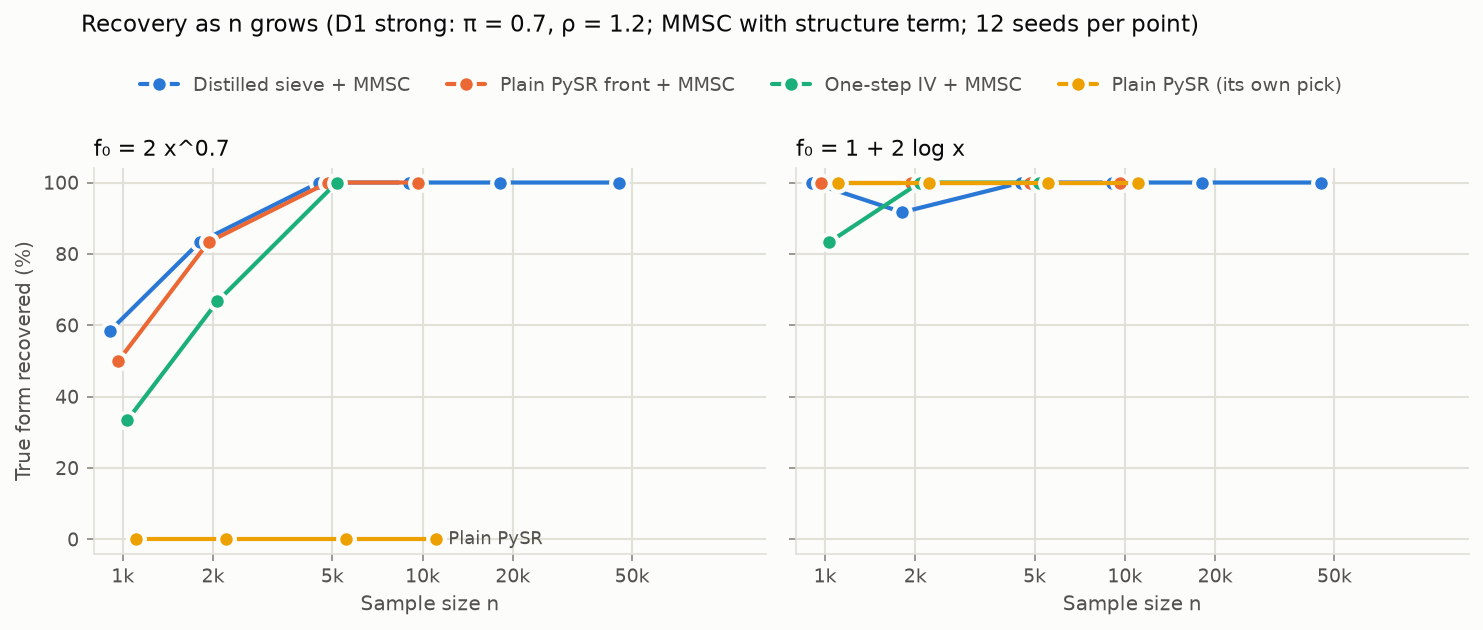
\includegraphics[width=\textwidth]{fig_nscale_light.png}
\caption{Recovery against sample size in the D1 strong setting ($\pi = 0.7$, $\rho = 1.2$), for the distilled, plain-PySR and one-step candidates scored by BIC + structure, and for plain PySR's own pick; 50 seeds per point at $n \le 5000$, 12 beyond.}
\label{fig:nscale}
\end{figure}

The instrument does its work when formulas are scored, not when they are generated. On the same runs (D1--D4), MMSC-BIC recovered the law from plain PySR's front about as often as from the IV-specific fronts: 52\%, against 47\% (one-step), 52\% (distilled) and 48\% (pooled). In the strong-endogeneity $n$-scaling cells, PySR's own pick recovered the power law in no run at any $n$ (50 seeds per cell up to $n = 5000$, 12 beyond), yet its front contained the true form in every run and the moment criterion selected it in 66--100\% of runs (Figure~\ref{fig:nscale}). Where PySR's own pick does get the form, its constants are biased: the log-law slope is 2.38--2.41 in D1, D2 and D4 against 2.00 with the moment criterion, and its in-sample errors are 5--16 times larger. IV-specific generators matter where endogeneity changes the shape of $\E[y \mid X]$: under simultaneity (D3) the plain front contains the true form in 25\% of runs, against 44--48\% for the one-step and distilled fronts. The cheap generators are also faster: over the full grid, whose samples reach $n = 50{,}000$, a median of 9 seconds per plain or distilled search against 61 for the one-step search (26 against 4 at $n = 2000$ in Section~\ref{sec:mc-first}).

A structure term is needed. BIC plus $0.5\,\ell_s\log m$ raised pooled recovery from 51\% to 60\% (Table~\ref{tab:rules}; 46 runs won, 8 lost; McNemar $p < 0.001$). In the $n$-scaling cells it gave 98--100\% recovery at $n = 5000$ (50 seeds) and 100\% from $n = 10{,}000$ for every generator. With BIC alone, recovery of $2x^{0.7}$ plateaus at 86--90\% at $n = 5000$ and 75--92\% from $10{,}000$ to $50{,}000$: the rest chose a near-duplicate such as $(xe^{x/\max(c, x)})^{0.7}$ or $x^{0.75}(xe^{-x} + 1.74)$, which has the same number of constants as the truth, differs from it only at small $x$, and is separated by its size, not by the moments. This is the case that falls under neither channel of \res{Theorem}{2} and that the per-node penalty resolves. The term costs recovery on the saturation law, whose true form $ax/(b + x)$ is long: pooled recovery in D1 fell from 42\% to 25\%; the templates of Section~\ref{sec:budget} more than repair that. HQIC (44\%), AIC (24\%) and the cross-fitted criterion (28\%) are worse than BIC; cross-fitting fails because over-parameterized formulas that contain the truth tie with it on held-out moments (\res{Theorem}{1}, Remark~4). Doubling $K$ changed nothing (16 runs won, 17 lost); kernel instruments were slightly better than splines (54\% against 51\%; 19 won, 6 lost; $p = 0.015$).

Distilled fronts select better than one-step fronts, and pooling does not help. Distilled fronts contain the true form more often than one-step fronts (74\% against 65\%) and hold fewer wrong formulas that outscore the truth under BIC (1.0 against 1.6 per run; at least one in 32\% against 44\% of runs). Pooling, a median of 28 candidates per run, raises coverage to 79\% but nearly triples these wrong formulas (2.9 per run), so recovery given coverage falls from 84\% to 72\% and the pooled set does not beat the distilled front alone. The library baseline's limit is coverage, not the IV logic: its Lasso path scored by the moment criterion recovers the log law in 100/100/92/75\% of runs in D1--D4 (against 28--52\% with cross-validated Lasso in the D1 and D2 cells of Section~\ref{sec:mc-baselines}), and given coverage it recovers 96\% of the time, but it contains the true form in only 35\% of runs because only the log law is in its library. Dropping \code{max} does not help: in paired comparisons no difference exceeded 3 runs ($p \ge 0.25$), and without \code{max} contrived winners use other operators.

Separation explains the selection failures, in a corrected form. The separation constant $\delta_L$ over all wrong trees was about zero in every cell and unrelated to recovery (Spearman 0.10), for two reasons: trees with more constants than $f_0$ approximate it arbitrarily well, and with a four-point instrument a tree with four constants can set the criterion to zero (\res{Proposition}{4}). The quantity that matters is the penalty-adjusted margin of~\eqref{eq:margin}, $\min_s[n\delta_s/\sigma_u^2 - (p_0 - p_s)\ln n]$ with the error variance $\sigma_u^2$ as the normalization $\sigma^2$ of~\eqref{eq:margin}, over wrong trees with $p_s \le p_0$, computed with the instruments the selection used on 20{,}000 noise-free draws, over the wrong formulas any run produced. Among runs whose candidates contained the true form it tracked recovery: Spearman 0.56 ($p < 0.001$) across 32 cells, 74\% recovery when the margin is positive and 23\% when it is not (Figure~\ref{fig:separation}). The margin is a worst case over the wrong formulas that were actually proposed, and the deviation terms of \res{Theorem}{2} explain why a small positive margin is not enough.

\begin{figure}[ht]
\centering
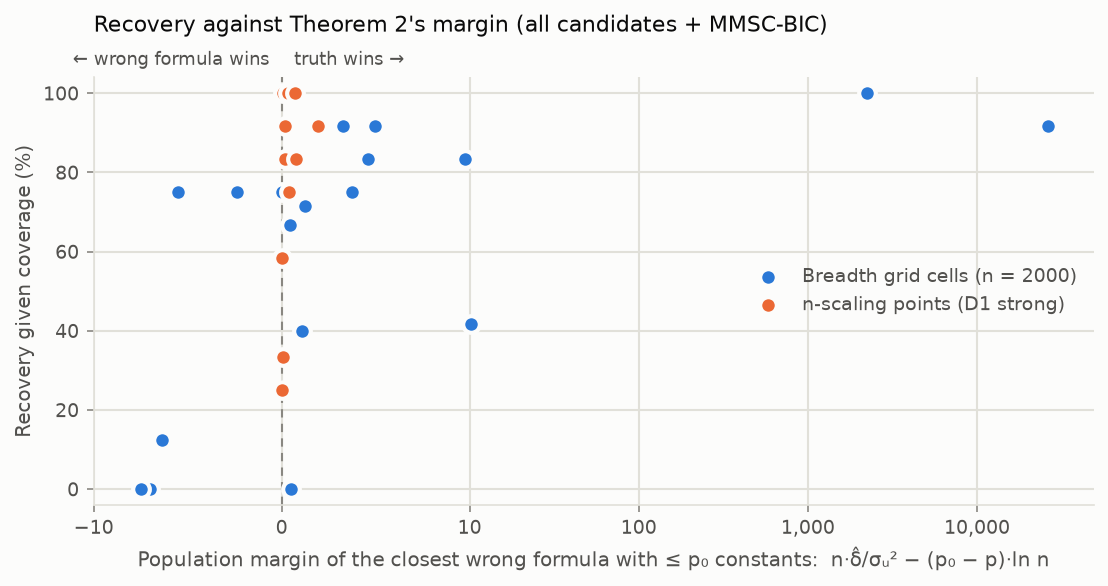
\includegraphics[width=\textwidth]{fig_separation_light.png}
\caption{Recovery given coverage against the penalty-adjusted separation margin, one point per cell of the breadth and $n$-scaling grids. Cells with a positive margin mostly recover the law; cells with a negative margin mostly do not.}
\label{fig:separation}
\end{figure}

The method fails in two places. The kink law was recovered in no pooled run, and no generator produced it in more than 33\% of runs; the saturation law appeared in 25--58\% of runs in D1--D4: search failures, taken up in Section~\ref{sec:budget}. Under the weak instrument (D5) recovery is 0--2\% for every law over 50 seeds; the selected formulas err by 0.3--1.0 sd in sample and 2.2--6.2 out of sample, and plain PySR's own pick is more accurate for two of the five laws in sample and four of five out of sample. The method should report weak identification there rather than a formula, and Section~\ref{sec:mc-ident} shows that it does. The control-function grid was inconclusive by design: with $\gamma = 0.45$ and $0.6$ control-function SR still never recovered the power law, but its log-law recovery rose to 83\% and 100\% because a larger $\gamma$ also increases the variance of $X$ given $Z$. On accuracy (D1--D4, pooled + structure), the median in-sample error is 0.040 against 0.129 for the sieve-2SLS curve; out of sample it is 0.074 when the form is recovered, 0.85 when it is not, and 0.76 for the sieve curve.

\subsection{Inference after selection}
\label{sec:mc-theory}

The remaining experiments test the theory on the saved fronts, with no new searches. The first tests \res{Theorem}{1(iii)}. For each run of the breadth grid at $n = 2000$, the law's own form and the formula selected by the pooled candidates with BIC + structure (when it has the true form) were estimated by two-step GMM on ten fresh samples and on the selection sample itself: 4{,}500 fits. Table~\ref{tab:inference} shows that on independent samples the intervals, the $J$ test and the AR sets are nominal, for the selected tree as for the oracle, and the standard errors are calibrated (the standard deviation of $\hat\theta - \theta_0$ across fresh samples is 0.84--1.00 times the mean reported standard error). On the selection sample, coverage of the constants drops to 83--90\% in D1--D3 (94\% with the discrete instrument): the post-selection distortion that splitting removes \citep{leebpotscher2005}. Under the weak instrument, Wald intervals for the oracle tree cover the constants 76\% of the time, the function at the median 68\% and the elasticity 64\%, and the $J$ test over-rejects, while the AR set at the true constants covers 97\%: AR inference survives weak identification of the constants, Wald inference does not. (A5)(a) held: every selected tree had a unique set of constants reproducing $f_0$.

\begin{table}[ht]
\centering\small
\caption{Inference after selection: coverage of nominal 95\% intervals and rejection rates of 5\% tests, 4{,}500 two-step GMM fits on the breadth-grid runs.}
\label{tab:inference}
\fittable{%
\begin{tabular}{@{}lccccc@{}}
\toprule
& Constants covered & $f$(median) & Elasticity & $J$ rejects & AR covers \\
\midrule
D1--D4, oracle, fresh samples & 93--95\% & 93--94\% & 92--96\% & 3--6\% & 93--97\% \\
D1--D4, selected tree, fresh samples & 92--98\% & 94--95\% & 92--94\% & 3--7\% & 93--97\% \\
D1--D4, selected tree, same sample & 83--94\% & 87--100\% & 88--96\% & 0--6\% & 94--97\% \\
D5 weak $Z$, true form, fresh samples & 76\% & 68\% & 64\% & 10\% & 97\% \\
\bottomrule
\end{tabular}}
\end{table}

\subsection{Candidates from one sample, selection on another}
\label{sec:mc-split}

This experiment tests \res{Corollary}{2.3} in the D1 strong setting, with the $n = 1000$ fronts and 12 seeds. When the same candidates are selected on five fresh samples of $n = 1000$ instead of the sample they were fitted to, the wrong candidates that outscore the truth fall from 1.92 to 1.37 per run (power law) and from 0.42 to 0.12 (log law), and recovery at equal selection size changes by $-2$ to $+25$ points across seven cells (median $+12$). But same-sample selection on the full $n = 2000$ with the structure term recovers more in all three BIC + structure cells (67\% against 47\%, 83\% against 72\%, 100\% against 92\%), because halving the sample halves the separation $n\delta_s$. Splitting is the right tool for inference, not for selection. The full table is in Appendix~\ref{app:tables}.

\subsection{The identification diagnostic}
\label{sec:mc-ident}

To test \res{Proposition}{5}, the report was run on every breadth-grid run, 630 after the 50-seed extension, with the pooled candidates and the BIC + structure selection on the run's own data ($\tau = 0.2$).

\begin{table}[ht]
\centering\small
\caption{The identification diagnostic on the 630 breadth-grid runs.}
\label{tab:ident}
\fittable{%
\begin{tabular}{@{}lcccc@{}}
\toprule
& Runs & Flagged (weakly identified or rejected) & Of which rejected & True form in $\Cc_\alpha$ \\
\midrule
D5 weak instrument, all runs & 250 & \textbf{100\%} & 16\% & 99\% \\
D1--D4, selection recovered the form & 257 & 4\% & 2\% & 99\% \\
D1--D4, statistical failure & 43 & 30\% & 7\% & 100\% \\
D1--D4, search failure & 80 & 54\% & 14\% & -- \\
\bottomrule
\end{tabular}}
\end{table}

Table~\ref{tab:ident} shows: coverage, \res{Proposition}{5}(a), across the 404 runs in which the true form was a candidate it is in the confidence set in 400 (99\%; nominal $\ge 95\%$). The weak instrument is always caught: in D5 the median first-stage $F$ is 3, 88\% of the candidates are not rejected, and the farthest member of the set differs from the selected formula by 0.8 sd (median); 84\% of the runs are reported ``weakly identified'' with the formulas the data also allow listed, and 16\% ``rejected''. False alarms are 4\% of the strong-instrument runs whose selection was right, the rate the 5\% AR level implies (at $\tau = 0.1$ it would be 14\%, with 58\% of the statistical failures caught instead of 30\%; Table~\ref{tab:tau}). Statistical failures, \res{Proposition}{5}(b): the true form was in the confidence set in all 43, and the diagnostic reports it as a different formula in 30\%; the other 70\% are near-duplicates within 0.2 sd of the truth, where the function is identified and only the tree is not minimal. Search failures: 54\% flagged, because the candidates that fit the moments disagree among themselves; the rest, mostly D3 with the kink and saturation laws, pass as ``identified'' because the wrong formula fits the moments and the other candidates agree with it, a case no diagnostic computed from the candidates can detect. With the discrete instrument (D4), 35\% of runs are ``weakly identified'' despite $F \approx 640$: with $K = 4$ moments the S test has little power, and the set contains formulas up to 0.13 sd away, \res{Proposition}{4} in the data.

\subsection{Discrete instruments}
\label{sec:mc-discrete}

\res{Proposition}{4} is visible in design D4 ($J = 4$), where the criterion has $K = 4$. On 20{,}000 noise-free draws, the wrong four-constant formula $c_0 + c_1\sqrt x + c_2x + c_3x^2$ fitted to the moments sets the criterion to $10^{-33}$--$10^{-32}$ for the power, kink and saturation laws while missing $f_0$ by 0.12, 0.15 and 0.42 standard deviations: \res{Proposition}{4}(a). For the log law the solution of the four moment equations lies outside the constant bound $\abs{c} \le 10$, so the bound, not the moments, keeps the criterion positive. Under D1's continuous instrument the same formula is separated from each law.
